\section{Towards a production ready software}

After the success of the prototype we were ready to design the production solution.
The production ready version of the system had to:
\begin{itemize}
  \item Support multiple circuit backends
  \item Separate all PhEDEx logic from circuit lifecycle management
  \item Provide a REST interface for external application control
  \item Provide a robust service to the application, regardless of 
  potential instabilities in the underlying network service
\end{itemize}

This redesign took the simple extension of the FileDownload agent to the 
software that is used today, whose class diagram is shown in Figure \ref{fig:class_diagram}.

\subsection{What was changed?}

\subsubsection{Circuit agent}

All of the logic initially inserted in the FileDownload agent has now been extracted and 
placed in the CircuitAgent, an agent directly extending the FileDownload agent. This opens 
the possibility of deploying the software in production and only using the circuit integration 
part with select sites. This is done by just by modifying a line in the PhEDEx config files.
Another advantage is that operators can quickly roll back to the normal FileDownload agent 
if the CircuitAgent misbehaves during integration

The CircuitAgent no longer contains the logic related to the lifecycle management of circuits.
This has been delegated to a new entity called the ResourceManager.

\subsubsection{ResourceManager}

The ResourceManager handles the lifecycle of circuits on behalf of PhEDEx and external programs.
It can be viewed as a stand-alone entity, as it can receive calls directly from PhEDEx or 
interact with external applications (like PanDA\cite{PANDA}) via a new REST API.

The new API supports the following calls:
\begin{itemize}
  \item createCircuit(to, from, lifetime, bandwidth): creates a circuit
  \item removeCircuit(to, from): tears down a circuit
  \item getInfo()
	\begin{itemize}
		\item RESOURCES: returns all info currently available (circuits active or expired
		\footnote{The queue of expired circuits is limited to the last 1000 entries})
		\item BACKEND\_TYPE: returns the circuit backend name used to provision circuits
		\item RESOURCE\_HISTORY: returns all info on expired circuits
		\item LINKS\_BLACKLISTED: returns all the links currently blacklisted
		\footnote{If a link is blacklisted, it means no circuit requests can be issued on it
		until it is whitelisted}
		\item ONLINE\_CIRCUIT, to, from: provides info on a specific active circuit
	\end{itemize}
\end{itemize}

Another important feature is that the ResourceManager can now use multiple circuit
providers via a plug-in system. Two circuit providers are supported at the moment: 
DYNES and NSI\cite{NSI}.
A third plug-in (Dummy) is provided for test purposes only.

The sequence diagram presented in Figure \ref{fig:sequence_diagram} shows the main events
at work in the software, as well as the interaction order  between them.

\begin{figure}[h]
  \centering
  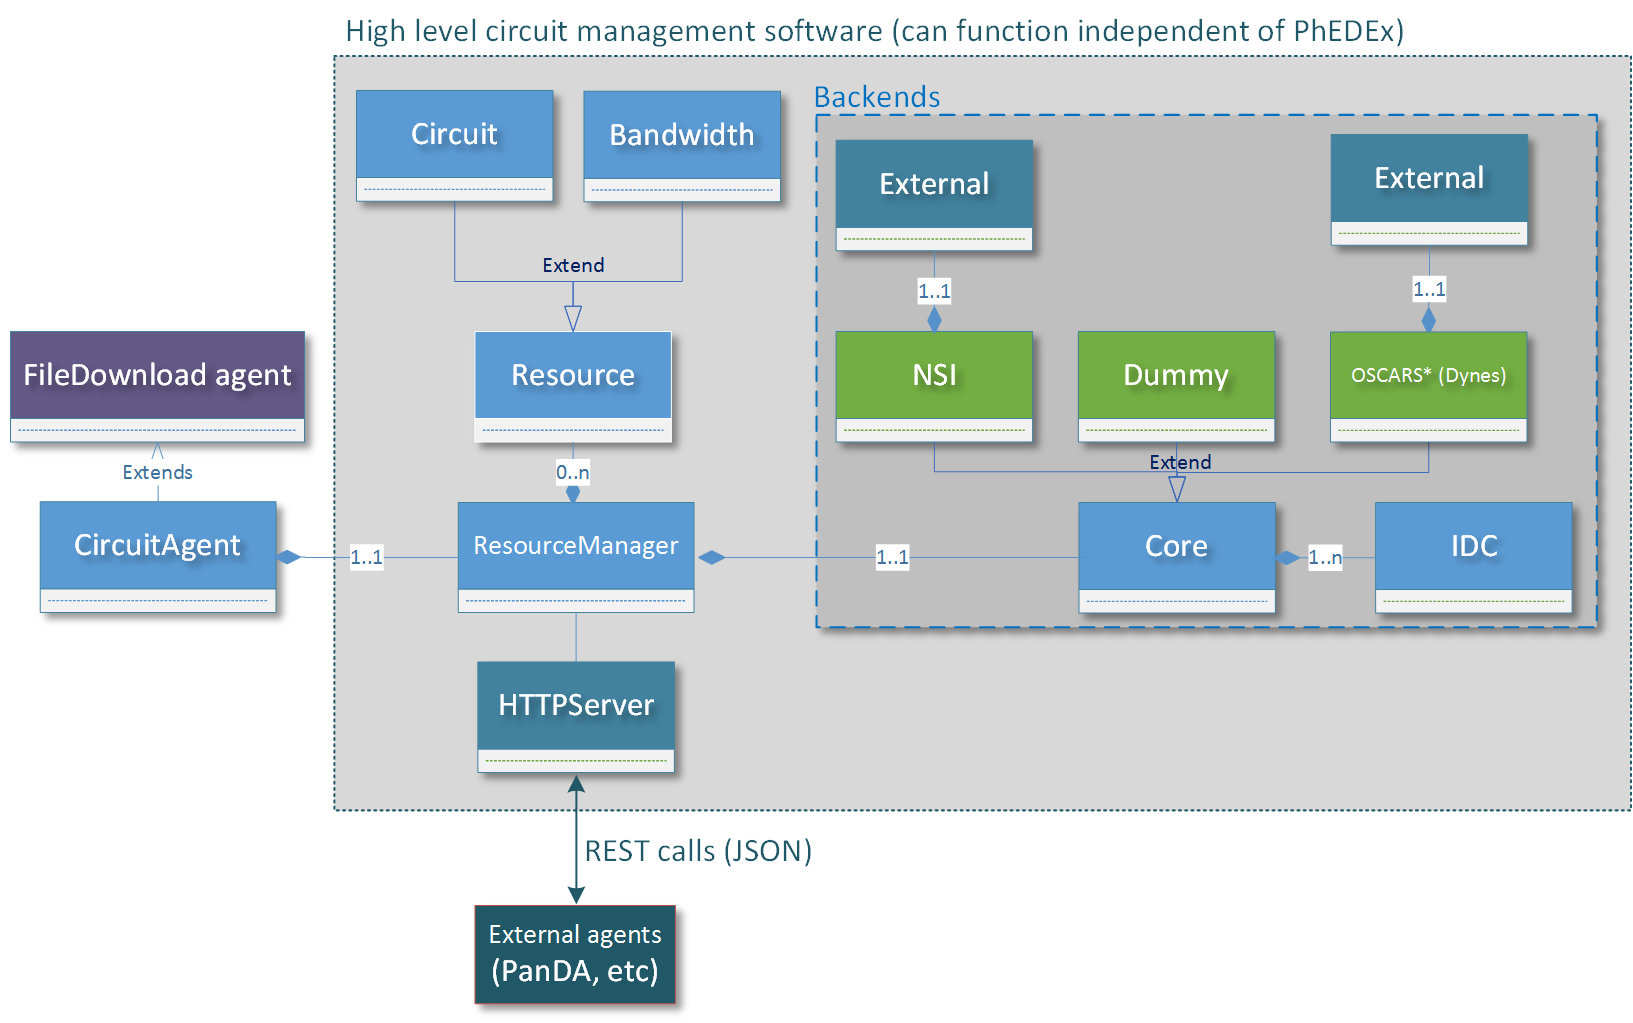
\includegraphics[width=0.95\textwidth]{Figures/Circuit_framework-class_diagram.png}
  \caption{Class diagram of the circuit management software integrated in PhEDEx}
  \label{fig:class_diagram}
\end{figure} 

\begin{figure}[h]
  \centering
  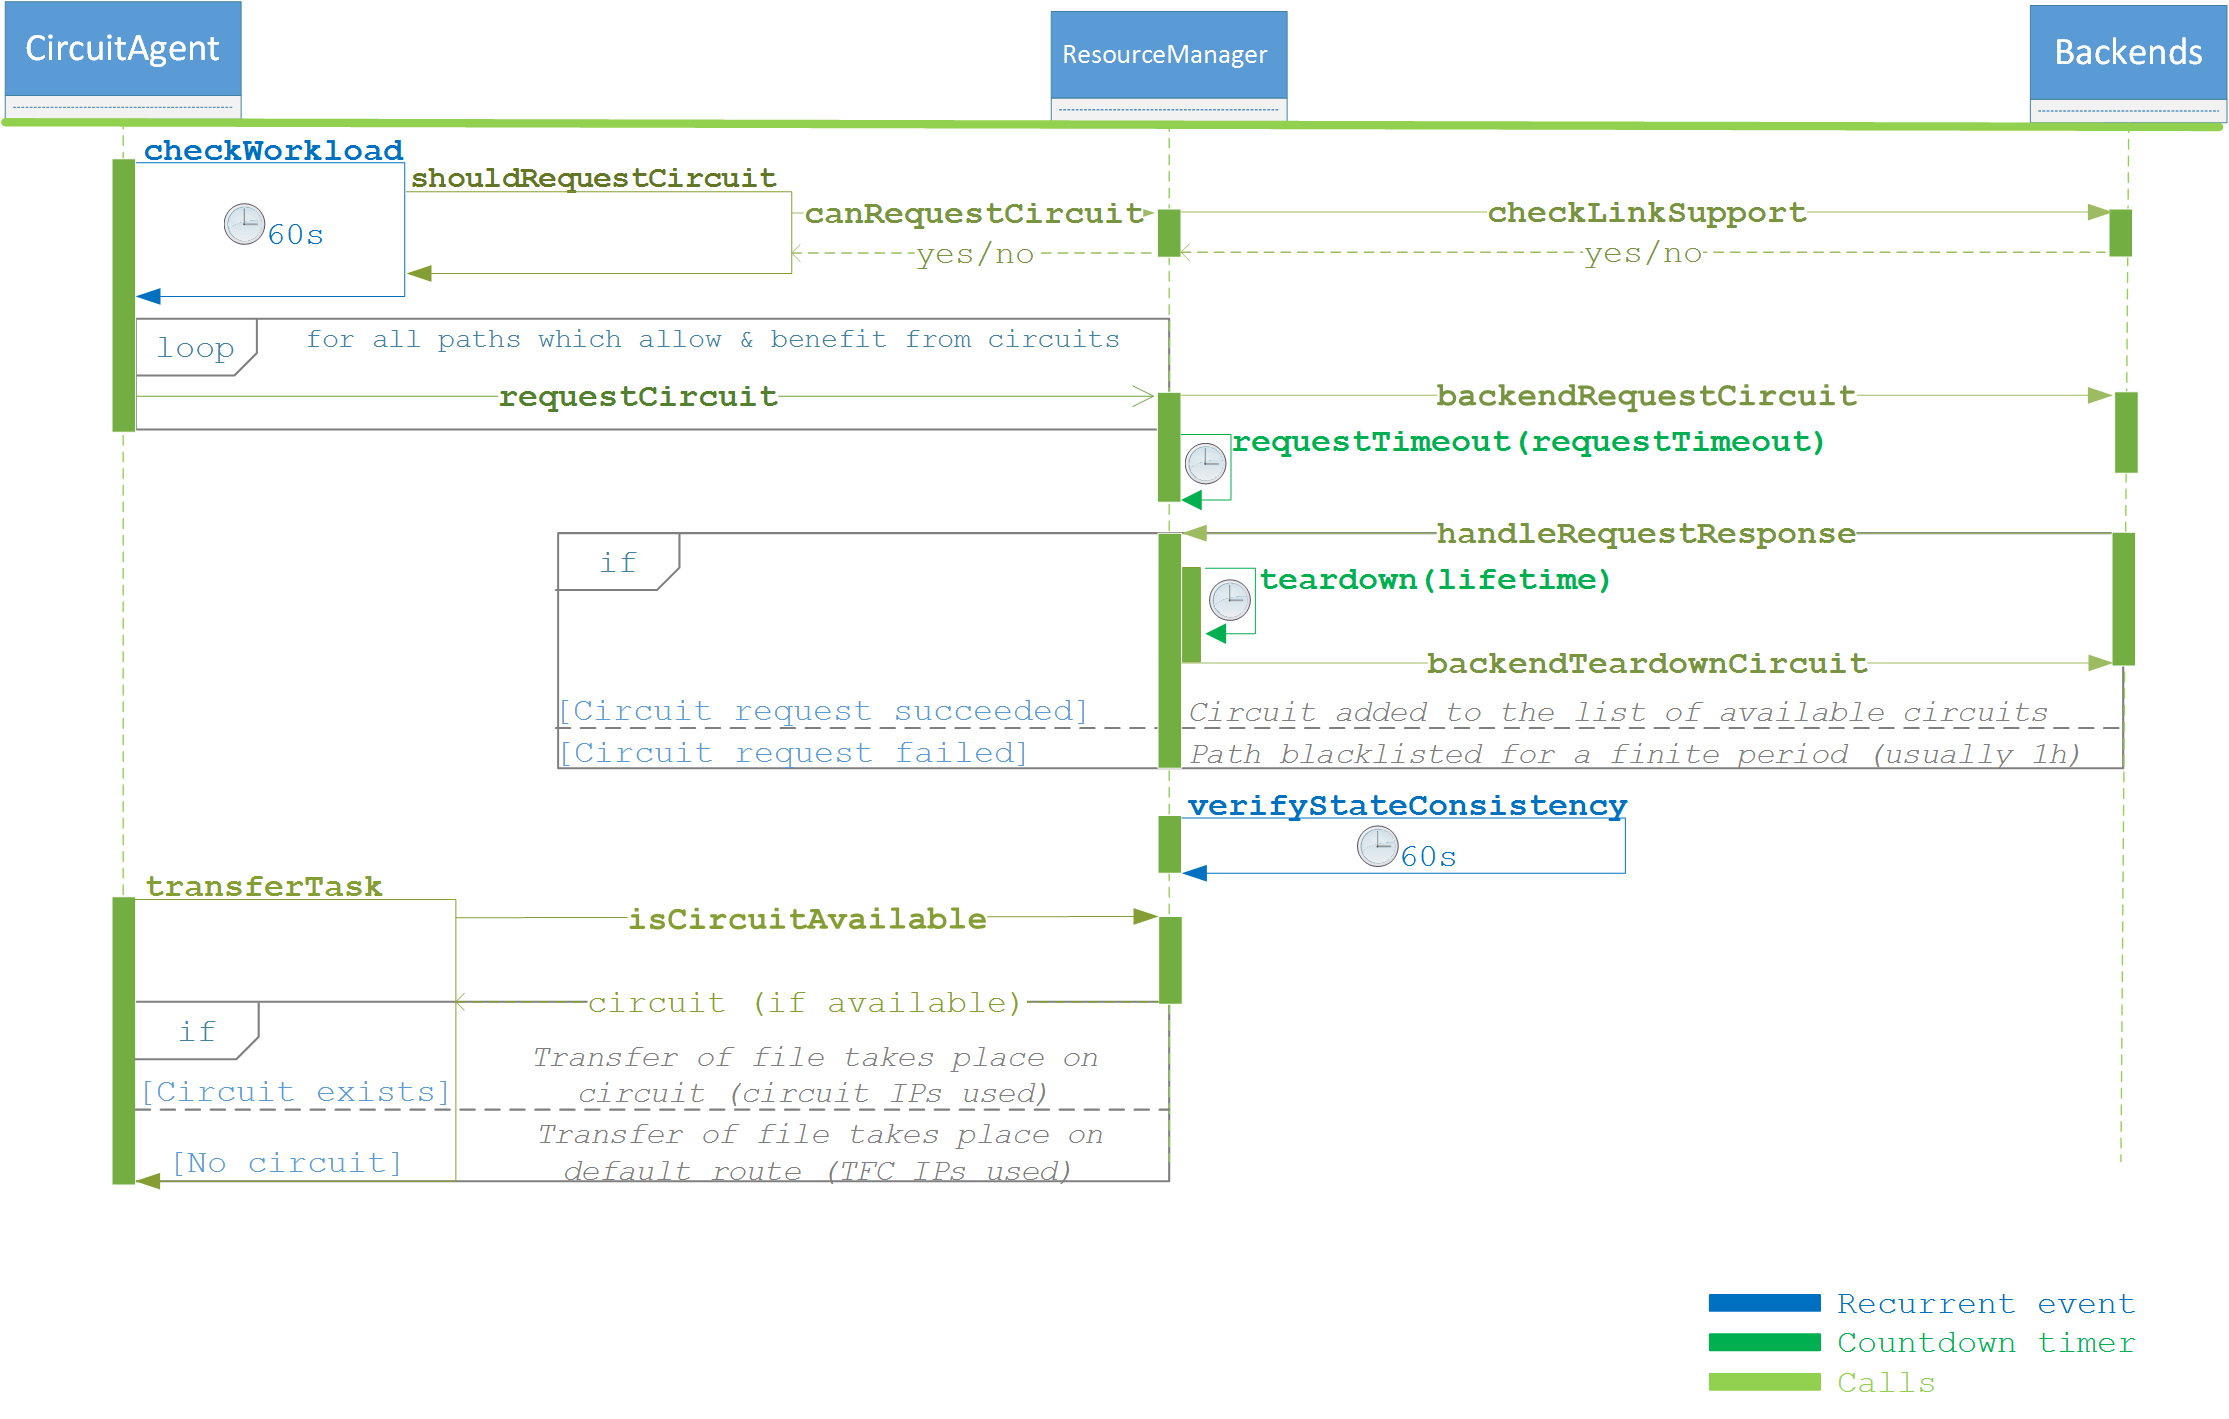
\includegraphics[width=0.95\textwidth]{Figures/Circuit_framework-sequence_diagram.png}
  \caption{Sequence diagram of the circuit management software integrated in PhEDEx}
  \label{fig:sequence_diagram}
\end{figure} 

\subsection{Circuit providers}

When ANSE began it was assumed it would use the DYNES infrastructure to provide Layer 3 circuits 
between a select number of sites. DYNES was regarded as a "dynamic network cyber-instrument"
and spanned over 40 US universities and 14 Internet2 connectors. It was based on the 
implementation of IDCP (Inter-Domain Circuit Protocol) developed by ESnet and Internet2 
(with cooperative development from GEANT and GLIF as well).

As official funding ended for DYNES, the lack of continued support forced a switch to different 
technologies. To this end, NSI was chosen as the replacement for DYNES as it is presently 
supported by many important network providers around the globe (ESnet, Internet2, GEANT, etc.)

\subsubsection{What is NSI?}

NSI stands for Network Service Interface and is defined as the interface between a
NS requestor agent and a NS provider agent, to request a transport connection.
The requestor could be a host, middleware or network provider, while the provider 
could be a home or campus network, or even a national infrastructure provider.

NSI provides different functionalities:
\begin{itemize}
  \item Resource management: Scheduling, reservation, instantiation, negotiation
  \item Resource information: Service discovery, topology exchange, monitoring, history, security
\end{itemize}

NSI\cite{NSI-CS2} supports both tree and chain models of service chaining, and it's effectively a two 
phase reservation system (Figure \ref{fig:NSI_RSM}).

\begin{itemize}
  \item First phase
	\begin{itemize}
		\item Reservation is made
		\item Availability is checked
		\item Resources are (temporarily) held
	\end{itemize}
  \item Second phase
	\begin{itemize}
		\item Requestor commits or aborts the reservation
		\item Should the requestor fail to act within a certain time limit, the reservation is released
	\end{itemize}
\end{itemize}

\begin{figure}[h]
  \centering
  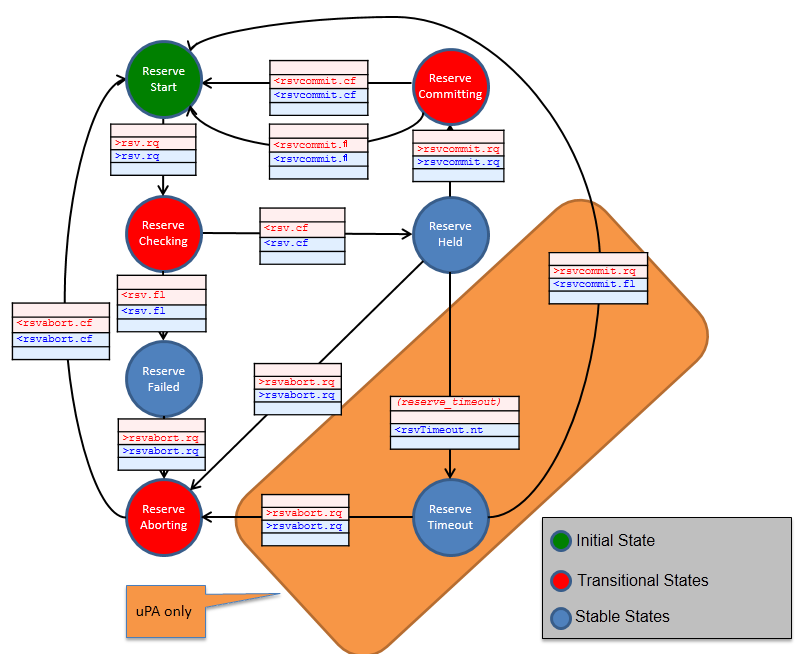
\includegraphics[width=0.95\textwidth]{Figures/NSI_RSM.png}
  \caption{The NSI Reservation State Machine}
  \label{fig:NSI_RSM}
\end{figure} 

The NSI plug-in implemented in our software uses an NSI CLI tool which was provided by ESnet.
